\documentclass[a4paper,11pt]{book}
\usepackage[magyar]{babel}
\usepackage[utf8]{inputenc}
\usepackage{graphicx}
\usepackage{amssymb,amsmath}
\usepackage{amsthm}
\usepackage{hyperref}
\usepackage{subcaption}
\usepackage{caption}
\usepackage{boondox-calo}
%\usepackage[caption=off]{subfig}
\usepackage[export]{adjustbox}
\usepackage{algorithm} 
\usepackage{algpseudocode} 
\usepackage[table]{xcolor}

\newtheorem{defn}{Def.}

\usepackage{etoolbox}
\AtBeginEnvironment{example}{\small\captionsetup[figure]{font=small}}
%\AtBeginEnvironment{proof}{\small}
\AtBeginEnvironment{problem}{\small\captionsetup[figure]{font=small}}

\newtheorem{example}{Példa}
\newtheorem{problem}{Feladat}

\renewenvironment{proof}
{\small \itshape Bizonyítás:\captionsetup[figure]{font=small}
}
{
	\hfill $\square$
	\vspace{2mm}
}

\newenvironment{remark}
{\small \itshape Megjegyzés:\captionsetup[figure]{font=small}
}
{
	
	\vspace{2mm}
}

\newenvironment{mathback}
{\small \itshape Matematikai háttér:\captionsetup[figure]{font=small}
}
{
			
	\vspace{2mm}
}

\newtheorem{defn2}{Definíció}

\usepackage{xcolor}

\newcommand{\acos}{\operatorname{acos}}
\newcommand{\asin}{\operatorname{asin}}
\newcommand{\atan}{\operatorname{atan}}
\newcommand{\diag}{\operatorname{diag}}
\newcommand{\rank}{\operatorname{rank}}
\newcommand{\atantwo}{\operatorname{atan2}}
\newcommand{\Span}[1]{\operatorname{span} \left\{ #1 \right\}}
\newcommand{\DoF}{\operatorname{DoF}}
\newcommand{\DoR}{\operatorname{DoR}}
\newcommand{\normalize}{\operatorname{normalize}}
\newcommand{\grad}{\operatorname{grad}}
\newcommand{\svd}{\operatorname{svd}}
\newcommand{\inv}{\operatorname{inv}}
%\newcommand{\dim}{\operatorname{dim}}
\renewcommand{\Im}[1]{\mathcal R({#1})}
\newcommand{\Ker}[1]{\mathcal N({#1})}
\newcommand{\Rot}[2]{\mathrm{Rot}(#1,#2)}
\newcommand{\Rotx}[1]{\mathrm{Rot}_x(#1)}
\newcommand{\Roty}[1]{\mathrm{Rot}_y(#1)}
\newcommand{\Rotz}[1]{\mathrm{Rot}_z(#1)}
\newcommand{\Tran}[1]{\mathrm{Tran}(#1)}
\newcommand{\Tranx}[1]{\mathrm{Tran}_x(#1)}
\newcommand{\Trany}[1]{\mathrm{Tran}_y(#1)}
\newcommand{\Tranz}[1]{\mathrm{Tran}_z(#1)}
\newcommand{\Trace}[1]{\mathrm{Tr}\left( #1 \right)}
\newcommand{\Normalize}[1]{\left( #1 \right)_{\mathrm{norm}}}
\newcommand{\minimize}[1]{\mathop{\mathrm{minimize}}_{#1} \ \ }
\newcommand{\subjectto}{\mathrm{subject \ to} \quad}
\newcommand{\T}{\top}
\newcommand{\DEG}{^{\circ}}

%\babelhyphenation{hi-\'a-nyos-an m\'er-n\"ok-\"ok meg-\'ert-\'es-\'e-ben link-ek-nek hoz-z\'á-juk}

\begin{document}

\author{Rezső Dezső, Prof. Emeritus}
\title{Bevezetés a rezsóológia elméletbe}
\date{\today}

\frontmatter
\maketitle
\tableofcontents

\mainmatter


\chapter*{Előszó}
\addcontentsline{toc}{chapter}{Előszó}

A könyv megszületését az Prof. Drexler Dániel motiválta. A cél pálinkafőzésre is alkalmas rezsó kifejlesztése, egyetemi alkalmazásának bevezetése.


Mélyebb érdeklődés esetén ajánljuk mátrixanalízis témába Rózsa Pál könyvét \cite{RozsaPalMatrix}, optimalizációs területen \cite{polyak1987introduction}, Bártfai Pál a lineáris algebra és az $n$-dimenziós geometria kapcsolatának rigorózus végigvezetését bemutató könyvét \cite{BartfaiNDimLinGeom}, stb.


\chapter*{Jelölések és rövidítések jegyzéke}
\addcontentsline{toc}{chapter}{Jelölések és rövidítések jegyzéke}


\subsection*{Jelölések}


\begin{tabular}{ll}
	Skalár értékek: & $a,b,c,\dots,\alpha,\beta,\gamma,\dots$ \\
	Oszlop/sor vektorok: & $\mathbf a,\mathbf b,\mathbf c,\dots$ \\
	Mátrixok: &$\mathbf A,\mathbf B, \mathbf C,\dots$\\
	Koordinátarendszerek (keretek), pontok: &$\mathrm A,\mathrm B, \mathrm C,\dots$\\
	Az $A$ pont koordinátái az $R$ keretben: &$\mathbf a^{(R)}$\\
	Az $O$ pontból a $P$ pontba mutató vektor: &$\overrightarrow{OP}$\\
	 \ \ ennek koordinátái az $R$ keretben: &$\overrightarrow{OP}^{(R)}$\\
	 Az $\mathbf u_1$, $\mathbf u_2$, $\mathbf u_3$ mátrixok által kifeszített & \\
	 \ \ $\{ \alpha_1\mathbf u_1+\alpha_2\mathbf u_2+... | \alpha_1\in\mathbb R, \alpha_2\in\mathbb R, ... \}$ & $\Span{\mathbf u_1,\mathbf u_2,\mathbf u_3,...}$ \\
	 \ \ tér: & \\
	 Az $\mathbf M$ mátrix képtere: &$\Im{\mathbf M}$\\
	 Az $\mathbf M$ mátrix nulltere: &$\Ker{\mathbf M}$
\end{tabular}

\subsection*{Rövidítések}

\begin{tabular}{ll}
	Szabadságfok (Degree of Freedom):& $\DoF$ \\
	Redundanciafok (Degree of Redundancy):& $\DoR$ \\
	Lineáris intERPoláció: & LERP \\
	Gömbi lineáris interpoláció (Spherical LERP): & SLERP \\
	Normalizált lineáris interpoláció (Normalized LERP): & NLERP \\
	Tool Center Point & TCP
\end{tabular}

\subsection*{Vektor és mátrix műveletek}

\begin{tabular}{ll}
	Az $f$ skalár függvény gradiense:& $\grad_{f}$\\
	
	A $\mathbf v$ vektor transzponáltja:& ${\mathbf v}^{\T}$\\
	
	A $\mathbf v$ vektor 2-es normája (hossza):& $||\mathbf v||$\\
	
	A $\mathbf v$ vektor normalizáltja (iránya):& $\Normalize{\mathbf v}$\\
	
	A $\mathbf v$ és $\mathbf w$ vektorok skaláris szorzata:& ${\mathbf v}^{\T}\cdot\mathbf w$\\
	
	A $\mathbf v$ és $\mathbf w$ vektorok vektoriális szorzata:& ${\mathbf v} \times\mathbf w$\\
	
	Az a mátrix, amelyet bármely $\mathbf w$ vektorral & \\
	 \ \ \ \ jobbról megszorozva $(\mathbf v\times \mathbf w)$ értékét kapjuk: & $\mathbf v\times$\\
	
	Az $\mathbf M$ mátrix $\mathbf M = \mathbf U \cdot \mathbf S \cdot \mathbf V^\T$ SVD felbontása:& $[\mathbf U,\mathbf S, \mathbf V] = \svd{(\mathbf M)}$\\
	
	Az $\mathbf M$ mátrix inverze:& ${\mathbf M}^{-1}$\\
	
	Az $\mathbf M$ mátrix transzponáltja:& ${\mathbf M}^{\T}$\\
	
	Az $\mathbf M$ mátrix determinánsa:& $\det{(\mathbf M)}$\\
	
	Az $\mathbf M$ mátrix ún. Moore-Penrose pszeudoinverze :& ${\mathbf M}^{+}$\\
	
	Az $\mathbf M$ mátrix ún. csillapított pszeudoinverze, & \\
	 \ \ \ \ $\rho$ csillapítással :& ${\mathbf M}^{\rho +}$\\ %TODO: biztosan jó lesz ez magyarul?
	
	Az $\mathbf M$ mátrix nyoma (főátlóbeli elemeinek összege):& $\Trace{\mathbf M}$\\
	
	A $\mathbf t$ irány körüli $\varphi$ szögű elfordulást leíró transzformáció:& $\Rot{\mathbf t}{\varphi}$\\
	
	Az $x$, $y$ vagy $z$ tengely körüli $\varphi$ & \\
	\hspace{15mm} szögű elfordulást leíró transzformáció:& $\Rotx{\varphi}$, $\Roty{\varphi}$, $\Rotz{\varphi}$ \\
	
	A $\mathbf d$ mértékű elmozdulást leíró transzformáció:& $\Tran{\mathbf d}$ \\
	
	Az $x$, $y$ vagy $z$ irányú $d$ & \\
	\hspace{15mm} nagyságú elmozdulást leíró transzformáció:& $\Tranx{d}$, $\Trany{d}$, $\Tranz{d}$ \\
	
	Az aktuális példában egyértelmű, vagy indifferens méretű & \\
	\hspace{15mm} vektorok, mátrixok jelölése: & $\begin{bmatrix}
		c_1 \\ c_2 \\ \vdots
	\end{bmatrix}$, $\begin{bmatrix}
		m_{11} & m_{12} & \dots \\
		m_{21} & m_{22} & \dots \\
		\vdots & \vdots &
	\end{bmatrix}$ \\

	A $t$ érték a következő értékeket veheti fel: $a\leq t\leq b$ & $t\in[a,b]$
	
\end{tabular}


\part{Bevezetés}

\chapter{Rezsó típusok}

\begin{figure}[ht!]
	\centering
	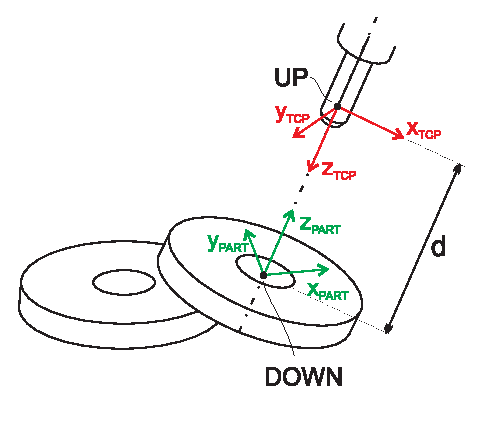
\includegraphics[width=0.7\linewidth]{img/trans_example-1}
	\caption{}
	\label{fig:transexample-1}
\end{figure}


\chapter{Algebrai áttekintés}

\part{Pálinkafőzés otthon}


\part{Soros kinematikai láncú rezsók modellezése}

\part{Rezsók dinamikai modellezése}


\backmatter
\bibliographystyle{IEEEtran}
\bibliography{bookbib}

\end{document}